% !TEX program = pdflatex
% !BIB pro%gram = bibtex
% !TEX encoding = UTF-8 Unicode
% !TEX spellcheck = en_us
\documentclass[10pt,sigconf]{acmart}

\usepackage{booktabs} % For formal tables

\graphicspath{{figure/}{figures/}}

% Copyright
%\setcopyright{none}
%\setcopyright{acmcopyright}
%\setcopyright{acmlicensed}
\setcopyright{rightsretained}
%\setcopyright{usgov}
%\setcopyright{usgovmixed}
%\setcopyright{cagov}
%\setcopyright{cagovmixed}


% DOI
\acmDOI{10.475/123_4}

% ISBN
\acmISBN{123-4567-24-567/08/06}

%Conference
\acmConference[CR for Nano'21]{AzuNet Seminar}{July 2021}{Lübeck, Germany} 
\acmYear{2021}
\copyrightyear{2021}

\acmPrice{15.00}


\begin{document}
\title{Computational Requirements for Nano-machines}
\titlenote{Produces the permission block, and copyright information}
%\subtitle{Extended Abstract}

\author{Melanie Badura}
\orcid{1234-5678-9012}
\affiliation{%
  \institution{Universität zu Lübeck}
  \streetaddress{Ratzeburger Allee 160}
  \city{Lübeck}  
  \postcode{23560}
}
\email{melanie.badura@student.uni-luebeck.de}




% The default list of authors is too long for headers}
\renewcommand{\shortauthors}{F. Lastname et al.}


\begin{abstract}
This paper is a shortpaper for "Computational Requirements for 
Nano-Machines: There is limited Space at the bottom".\footnote{}
\end{abstract}

%
% The code below should be generated by the tool at
% http://dl.acm.org/ccs.cfm
% Please copy and paste the code instead of the example below. 
%
\begin{CCSXML}
<ccs2012>
 <concept>
  <concept_id>10010520.10010553.10010562</concept_id>
  <concept_desc>Computer systems organization~Embedded systems</concept_desc>
  <concept_significance>500</concept_significance>
 </concept>
 <concept>
  <concept_id>10010520.10010575.10010755</concept_id>
  <concept_desc>Computer systems organization~Redundancy</concept_desc>
  <concept_significance>300</concept_significance>
 </concept>
 <concept>
  <concept_id>10010520.10010553.10010554</concept_id>
  <concept_desc>Computer systems organization~Robotics</concept_desc>
  <concept_significance>100</concept_significance>
 </concept>
 <concept>
  <concept_id>10003033.10003083.10003095</concept_id>
  <concept_desc>Networks~Network reliability</concept_desc>
  <concept_significance>100</concept_significance>
 </concept>
</ccs2012>  
\end{CCSXML}


\ccsdesc[500]{Computer systems organization~Embedded systems}
\ccsdesc[300]{Computer systems organization~Redundancy}
\ccsdesc{Computer systems organization~Robotics}
\ccsdesc[100]{Networks~Network reliability}

% We no longer use \terms command
%\terms{Theory}

\keywords{ACM proceedings}


\maketitle

\section{Introduction}

Refer to \verb|acmart.pdf| \cite{veytsmanlatex} (\url{https://www.ctan.org/pkg/acmart}, \url{http://www.acm.org/publications/proceedings-template}) for additional examples and instructions.

\section{Mittelteil?}

\section{Conclusion}

\subsection{Subsection}

Lorem ipsum dolor sit amet, consectetur adipiscing elit.
Sed aliquam nisl turpis, sit amet mollis leo accumsan vel.
Donec semper turpis dui, a porttitor lorem tincidunt id.
Phasellus gravida, purus non faucibus euismod, lectus tortor maximus elit, vestibulum lobortis purus turpis non urna.
Fusce feugiat lectus ut massa molestie, non interdum augue porta.
Nunc dapibus odio nec neque cursus, ut lacinia velit rutrum.
Duis tempor nulla velit, sed pellentesque nunc imperdiet ut.
Phasellus eget hendrerit neque.
Suspendisse aliquet nulla id sem aliquam aliquam sed a orci.
Duis sem est, hendrerit nec porttitor sit amet, maximus sed nulla.
Suspendisse et dictum massa.
Morbi non diam nec orci sodales eleifend.
Etiam eget finibus purus, a malesuada ipsum.
Nullam ac nisi nec elit faucibus aliquet.
Nulla feugiat velit sed sodales eleifend.
Donec orci nulla, viverra et mi in, sagittis egestas urna.

\begin{figure}[htbp]
  \centering
  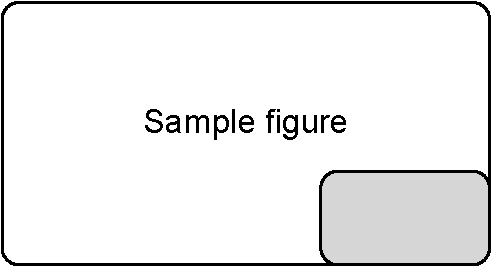
\includegraphics[scale=0.5]{sample-figure}
  \caption{Sample figure}
  \label{fig:sample}
\end{figure}




\bibliographystyle{acm}
\bibliography{sigproc} 

\end{document}
